Dieses Kapitel beschäftigt sich mit der Analyse und der Bewertung von den eingeführten Verfahren aus den Kapiteln \ref{chp:sichtpruefungDurchLichtstreuung} und \ref{chp:deflektometrischeRegistrierung} zur Auswertung von Oberflächeninformationen spiegelnder Prüfobjekte.
Im Anschluss an der Beschreibung der Ergebnisse der einzelnen Verfahren soll eine Diskussion und ein direkter Vergleich anhand bestimmter Kriterien erfolgen.

%Sichtprüfung durch Lichtstreuung
{
	\FloatBarrier
    \section{Sichtprüfung durch Lichtstreuung}
    \label{sec:ergebnisseSichtpruefungDurchLichtstreuung}
    Das Verfahren \glqq Sichtprüfung durch Lichtstreuung\grqq ~wurde in Kapitel \ref{chp:sichtpruefungDurchLichtstreuung} eingeführt und lässt insbesondere kleine Defekte auf spiegelnden Oberflächen sichtbar werden.
%TODO mehr Allgemeines über das Verfahren? -> Ich denke nicht nötig
Die Parameter zur Erzeugung der Muster nach Gleichung \ref{eq:impulsStreifenmuster} können in Tabelle \ref{tab:paramSichtpruefung} abgelesen werden.

\begin{table}[H]
	\centering
	\begin{tabular}{lll}
		\hline 
		\textbf{Beschreibung} & \textbf{Name} & \textbf{Wert} \\ 
		\hline 
		Tastgrad (beeinflusst die Streifenbreiten) & $D$ & $\tfrac{2}{5}$ \\ 
		Amplitude (beeinflusst die Helligkeit) & $A_m$ & 127.5 \\ 
		Kontrast & $C_m$ & 1.0 \\ 
		Anzahl Perioden des Musters & $N_p$ & 128 \\
		Anzahl Phasenverschiebungen & $N_{shift}$ & 16 \\ 
		Bildschirmbreite (in Pixel) & \acrshort{lwidth} & 1920 \\
		Bildschirmhöhe (in Pixel) & \acrshort{lheight} & 1080 \\ 
		\hline 
	\end{tabular}
	\caption{Parameter des Verfahrens}
	\label{tab:paramSichtpruefung}
\end{table}

\noindent
Durch diese Parameter erhält man eine Sequenz aus 16 Mustern die auf einem LCD-Bildschirm angezeigt und anschließend durch eine Kamera aufgenommen werden können.
Zur Kodierung der Oberfläche werden insgesamt 256 Helligkeitsstufen auf die Oberfläche abgebildet.
Zur Verbesserung der Ergebnisse werden die verwendeten Aufbauten durch geeignete Abschirmungen vor Fremdlicht geschützt.

% Durchlichtauswertung
{
	\FloatBarrier
    \subsection{Durchlichtauswertung}
    \label{sub:durchlichtAuswertungLichtstreuung}
    Zunächst wird für dieses Verfahren die Analyse mit der Durchlichtauswertung durchgeführt.
Aus dem Grund werden für die folgenden Bilder nur transparente Brillengläser untersucht.
In Abbildung \ref{tikz:abbStreifenaufnahmen} werden einzelne Aufnahmen der Brillengläser, bei Verwendung des Aufbaus aus dem linken Teilbild aus Abbildung \ref{tikz:abbAufbauFotos}, dargestellt.
Dabei wurden die Brillengläser auf eine dunkle Halterung gelegt, welche im linken Teilbild aus Abbildung \ref{tikz:abbAufbauFotos} über dem Bildschirm zu erkennen ist.

% Abbildung: Streifenaufnahmen
{
	\begin{figure}[H]
		\centering
		\begin{adjustbox}{width=\textwidth}
	\begin{tikzpicture}[every node/.style={inner sep=0,outer sep=0}]
		% Bilder
		\node [anchor=north west] (img1) at (0,0) {\includegraphics[frame,width=.31\textwidth]{05_ergebnisse/ergSichtpruefungDurchLichtstreuung/durchlichtAuswertungLichtstreuung/figures/gefärbtesBrillenglas2_rotiert_Bild}};
		\node [anchor=north west] (img2) at (0.345\textwidth,0) {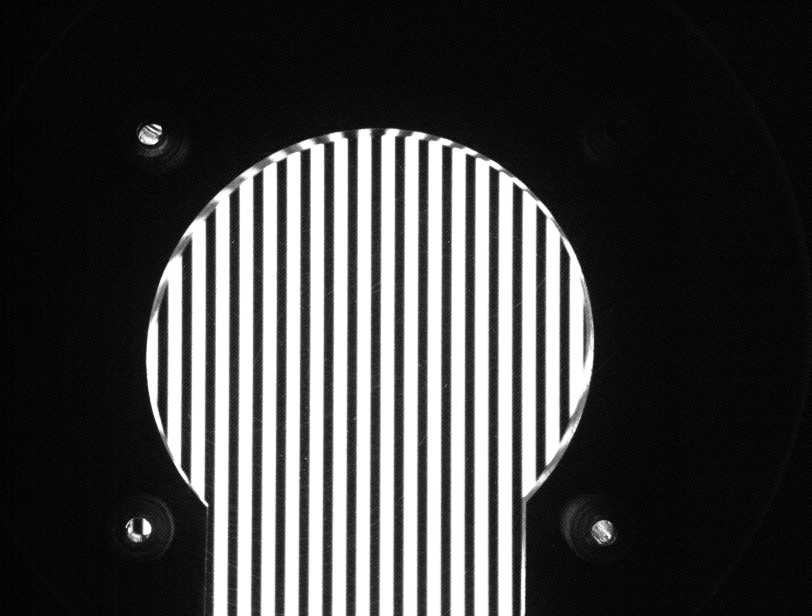
\includegraphics[frame,width=.31\textwidth]{05_ergebnisse/ergSichtpruefungDurchLichtstreuung/durchlichtAuswertungLichtstreuung/figures/polierfehler}};
		\node [anchor=north west] (img3) at (0.69\textwidth,0) {\includegraphics[frame,width=.31\textwidth]{05_ergebnisse/ergSichtpruefungDurchLichtstreuung/durchlichtAuswertungLichtstreuung/figures/HS_Beschädigung}};
		
		% Captions
		\node [below=0.2cm of img1] (cap1) {Brillenglas 1};
		\node [below=0.2cm of img2] (cap2) {Brillenglas 2};
		\node [below=0.2cm of img3] (cap3) {Brillenglas 3};			
	\end{tikzpicture}
\end{adjustbox}
\caption[Aufnahmen der Streifenmuster beim Durchlichtverfahren]{Aufnahmen der Streifenmuster beim Durchlichtverfahren}
		\label{tikz:abbStreifenaufnahmen}
	\end{figure}
}

%TODO Nutzen?
%\noindent
%Das Brillenglas 1 aus Abbildung \ref{tikz:abbStreifenaufnahmen} ist ein polarisierendes Sonnenbrillenglas.
%Das bedeutet, dass die Brille das auftreffende Licht je nach Polarisierung des Lichts deutlich stärker reflektiert.
%Somit gelangt nahezu nur noch Licht in einer speziellen Polarisation durch das Glas.
%Diese Eigenschaft kann man für die Spiegelbildauswertung nutzen um den Rückseitenreflex (vgl. Abschnitt \ref{sec:spiegelndeOberflaechen}) zu minimieren.

\noindent
Durch Anwendung des Verfahrens \glqq Sichtprüfung durch Lichtstreuung\grqq erhält man für die drei Brillengläser folgende Bilder:

% Abbildung: Ergebnis der Sichtprüfung durch Lichtstreuung
{
	\begin{figure}[H]
		\centering
		\begin{adjustbox}{width=\textwidth}
	\begin{tikzpicture}[every node/.style={inner sep=0,outer sep=0}]
		% Bilder
		\node [anchor=north west] (img1) at (0,0) {\includegraphics[frame,width=.31\textwidth]{05_ergebnisse/ergSichtpruefungDurchLichtstreuung/durchlichtAuswertungLichtstreuung/figures/gefärbtesBrillenglas2_rotiert_sichtpruefungLichtstreuung}};
		\node [anchor=north west] (img2) at (0.345\textwidth,0) {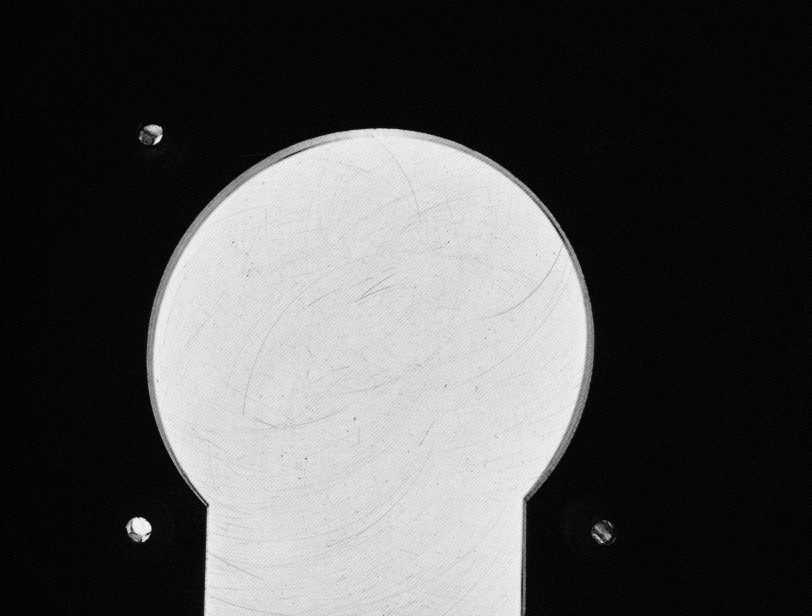
\includegraphics[frame,width=.31\textwidth]{05_ergebnisse/ergSichtpruefungDurchLichtstreuung/durchlichtAuswertungLichtstreuung/figures/polierfehler_ergebnis}};
		\node [anchor=north west] (img3) at (0.69\textwidth,0) {\includegraphics[frame,width=.31\textwidth]{05_ergebnisse/ergSichtpruefungDurchLichtstreuung/durchlichtAuswertungLichtstreuung/figures/HS_Beschädigung_ergebnis}};
		
		% Captions
		\node [below=0.2cm of img1] (cap1) {Brillenglas 1};
		\node [below=0.2cm of img2] (cap2) {Brillenglas 2};
		\node [below=0.2cm of img3] (cap3) {Brillenglas 3};			
	\end{tikzpicture}
\end{adjustbox}
\caption[Ergebnisbilder des Verfahrens \glqq Sichtprüfung durch Lichtstreuung\grqq]{Ergebnisbilder des Verfahrens \glqq Sichtprüfung durch Lichtstreuung\grqq}
		\label{tikz:abbCombinePatternPictures}
	\end{figure}
}

\noindent
Um die Bilder aus Abbildung \ref{tikz:abbCombinePatternPictures} zu erzeugen wurde als Verknüpfungsmethode des  Verfahrens die betragsmäßige Differenz gewählt, um einen hohen Kontrast zwischen der Halterung und dem sichtbaren Bereich des Brillenglases zu erzeugen.
Durch Anwendung einer Kontrastverbesserung in lokalen Bereichen des Bildes und geeigneter Kennlinientransformationen können die Bilder nachbearbeitet werden, um die Kratzer und Eingravierungen in der Oberfläche besser zu erkennen:

% Abbildung: Nachbearbeitung der Ergebnisbilder
{
	\begin{figure}[H]
		\centering
		\begin{adjustbox}{width=\textwidth}
	\begin{tikzpicture}[every node/.style={inner sep=0,outer sep=0}]
		% Bilder
		\node [anchor=north west] (img1) at (0,0) {\includegraphics[width=.31\textwidth]{05_ergebnisse/ergSichtpruefungDurchLichtstreuung/durchlichtAuswertungLichtstreuung/figures/gefärbtesBrillenglas2_rotiert_verbessert_Norm_LookUp}};
		\node [anchor=north west] (img2) at (0.345\textwidth,0) {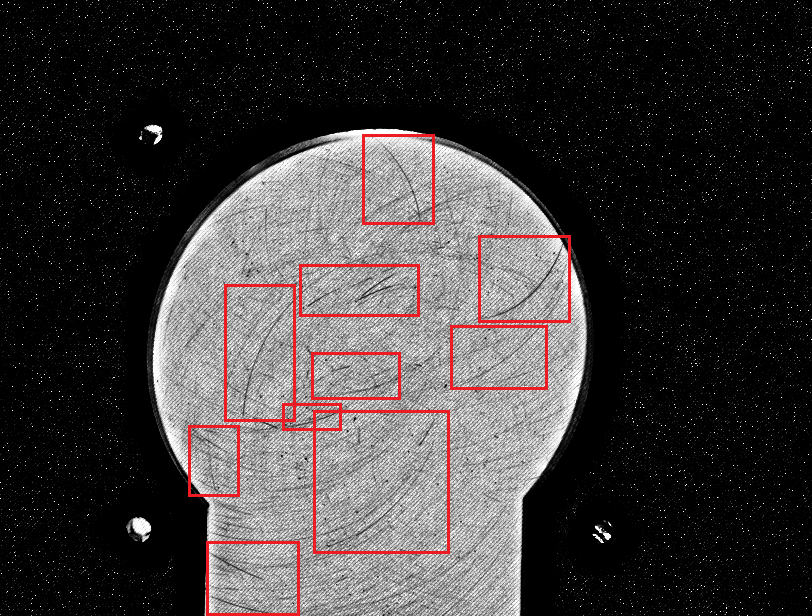
\includegraphics[width=.31\textwidth]{05_ergebnisse/ergSichtpruefungDurchLichtstreuung/durchlichtAuswertungLichtstreuung/figures/polierfehler_ergebnis_verbessert}};
		\node [anchor=north west] (img3) at (0.69\textwidth,0) {\includegraphics[width=.31\textwidth]{05_ergebnisse/ergSichtpruefungDurchLichtstreuung/durchlichtAuswertungLichtstreuung/figures/HS_Beschädigung_ergebnis_verbessert}};
		
		% Captions
		\node [below=0.2cm of img1] (cap1) {Brillenglas 1};
		\node [below=0.2cm of img2] (cap2) {Brillenglas 2};
		\node [below=0.2cm of img3] (cap3) {Brillenglas 3};			
	\end{tikzpicture}
\end{adjustbox}
\caption[Verbesserung der Ergebnisbilder]{Verbesserung der Ergebnisbilder. In Grün: Gravur der Brillenglaskennzeichnung. In Rot: Kratzer und ähnliche Beschädigungen der Oberfläche.\footnotemark}
		\label{tikz:abbNachbearbeitung}
	\end{figure}
	\footnotetext{Es wurde nur eine Auswahl von Fehlstellen markiert, um die Übersicht beizubehalten.}
}

\noindent
In den einzelnen Teilbildern aus Abbildung \ref{tikz:abbNachbearbeitung} kann man in den markierten Bereichen Fehlstellen bzw. Gravuren als dunkle Formen erkennen.
}

% Spiegelbildauswertung
{
	\FloatBarrier
    \subsection{Spiegelbildauswertung}
    \label{sub:spiegelbildAuswertungLichtstreuung}
    Nachdem das Verfahren für die Durchlichtauswertung Fehlstellen auf transparenten Objekten sichtbar machen konnte, stellt man sich die Frage, ob ähnliche Ergebnisse auch für nicht-transparente spiegelnde Objekte erzielt werden können.
Für diese Objekte wird das Verfahren mit der Spiegelbildauswertung durchgeführt.
Hierfür wählt man den Aufbau aus dem rechten Teilbild aus Abbildung \ref{tikz:abbAufbauFotos}.

\p
Für einen Vergleich der Spiegelbildauswertung zur Durchlichtauswertung für transparente Prüfobjekte wird das Brillenglas 1 (siehe linkes Teilbild aus Abbildung \ref{tikz:abbStreifenaufnahmen}) gewählt, da es durch ein polarisierendes Sonnenbrillenglas ist.
Das bedeutet, dass das Brillenglas das auftreffende Licht je nach Polarisierung des Lichts deutlich stärker reflektiert.
Somit gelangt nahezu nur noch Licht mit einer speziellen Polarisation durch das Glas.
Diese Eigenschaft kann man für die Spiegelbildauswertung nutzen um den Rückseitenreflex (vgl. Abschnitt \ref{sec:spiegelndeOberflaechen}) zu minimieren.
Die weiteren Objekte sind spiegelnde Keramikbruchstücke.

% Abbildung: Streifenaufnahmen
{
	\begin{figure}[H]
		\centering
		\begin{adjustbox}{width=\textwidth}
	\begin{tikzpicture}[every node/.style={inner sep=0,outer sep=0}]
		% Bilder
		\node [anchor=north west] (img1) at (0,0) {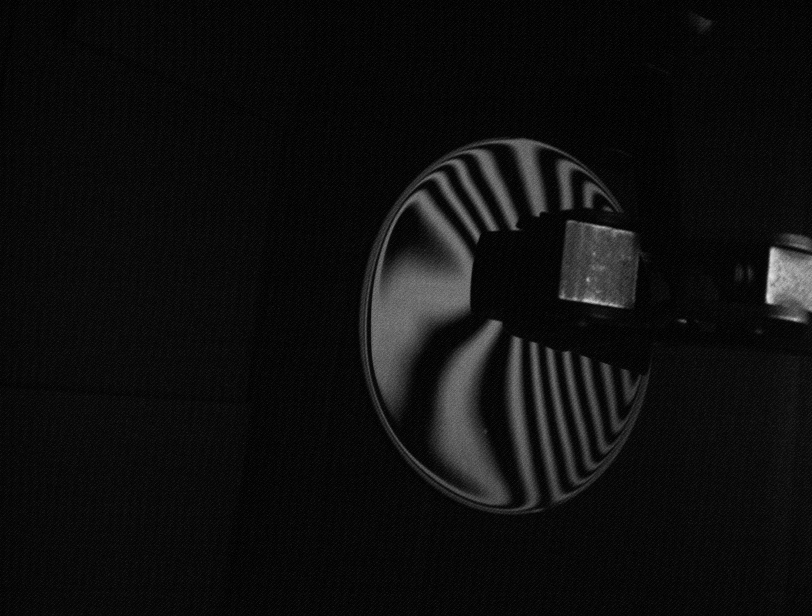
\includegraphics[width=.31\textwidth]{05_ergebnisse/ergSichtpruefungDurchLichtstreuung/spiegelbildAuswertungLichtstreuung/figures/brillenglas_1_beleuchtetImpuls}};
		\node [anchor=north west] (img2) at (0.345\textwidth,0) {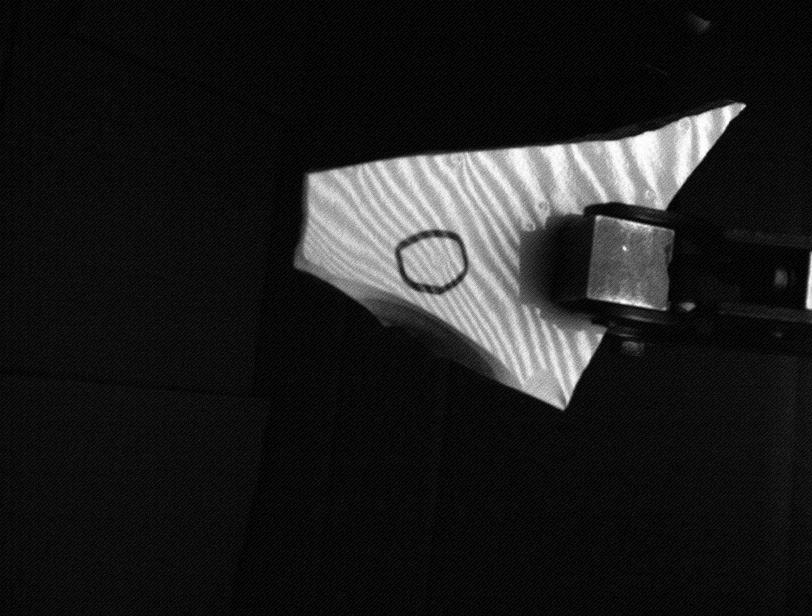
\includegraphics[width=.31\textwidth]{05_ergebnisse/ergSichtpruefungDurchLichtstreuung/spiegelbildAuswertungLichtstreuung/figures/keramikObjekt_1_beleuchtetImpuls}};
		\node [anchor=north west] (img3) at (0.69\textwidth,0) {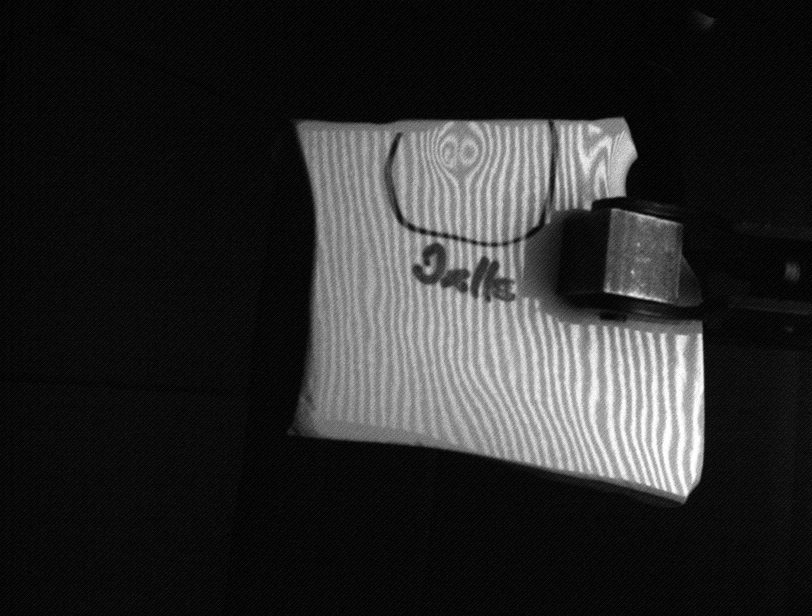
\includegraphics[width=.31\textwidth]{05_ergebnisse/ergSichtpruefungDurchLichtstreuung/spiegelbildAuswertungLichtstreuung/figures/keramikObjekt_2_beleuchtetImpuls}};
		
		% Captions
		\node [below=0.2cm of img1] (cap1) {Brillenglas 1};
		\node [below=0.2cm of img2] (cap2) {Keramikobjekt 1};
		\node [below=0.2cm of img3] (cap3) {Keramikobjekt 2};			
	\end{tikzpicture}
\end{adjustbox}
\caption[Aufnahmen der Streifenmuster bei der Spiegelbildauswertung]{Aufnahmen der Streifenmuster bei der Spiegelbildauswertung}
		\label{tikz:abbStreifenaufnahmenSpLichtstreuung}
	\end{figure}
}

\noindent
Durch Anwendung des Verfahrens \glqq Sichtprüfung durch Lichtstreuung\grqq ~erhält man für die drei Prüfobjekte folgende Bilder:

% Abbildung: Ergebnis der Sichtprüfung durch Lichtstreuung
{
	\begin{figure}[H]
		\centering
		\begin{adjustbox}{width=\textwidth}
	\begin{tikzpicture}[every node/.style={inner sep=0,outer sep=0}]
		% Bilder
		\node [anchor=north west] (img1) at (0,0) {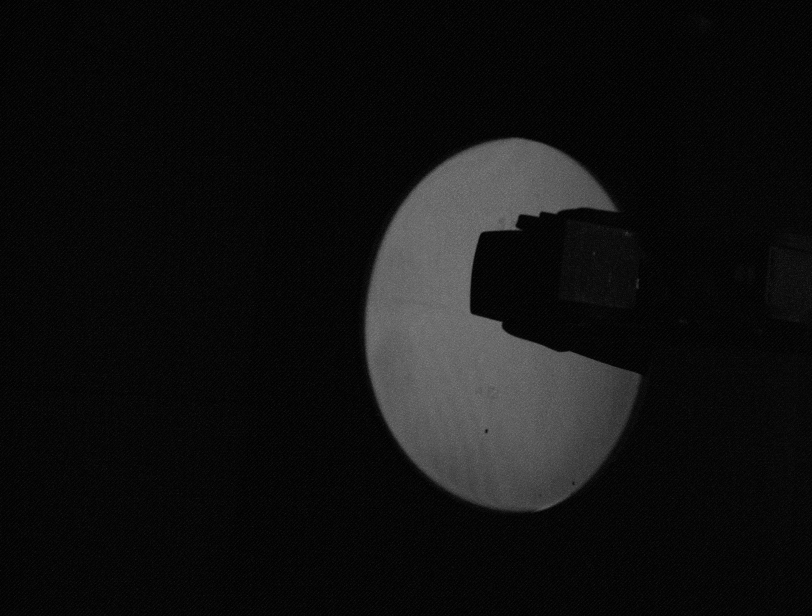
\includegraphics[width=.31\textwidth]{05_ergebnisse/ergSichtpruefungDurchLichtstreuung/spiegelbildAuswertungLichtstreuung/figures/brillenglas_1_combinePattern}};
		\node [anchor=north west] (img2) at (0.345\textwidth,0) {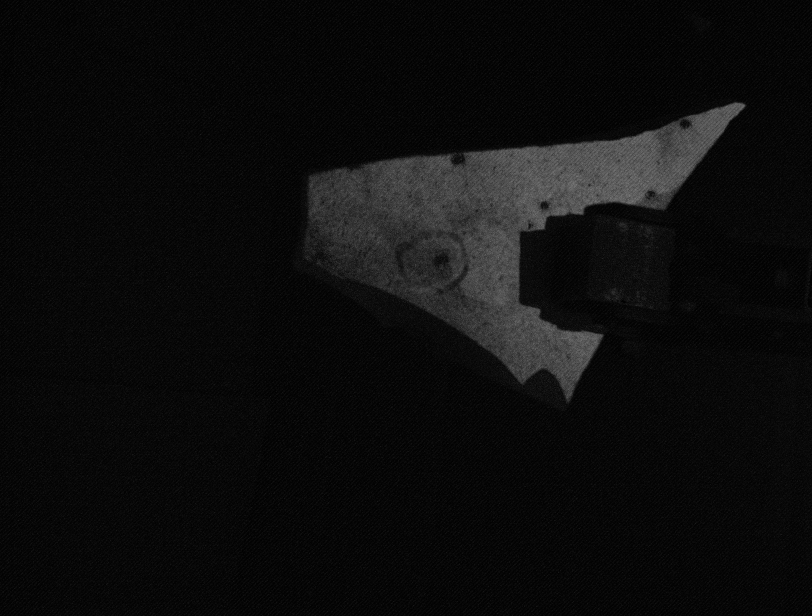
\includegraphics[width=.31\textwidth]{05_ergebnisse/ergSichtpruefungDurchLichtstreuung/spiegelbildAuswertungLichtstreuung/figures/keramikObjekt_1_combinePattern}};
		\node [anchor=north west] (img3) at (0.69\textwidth,0) {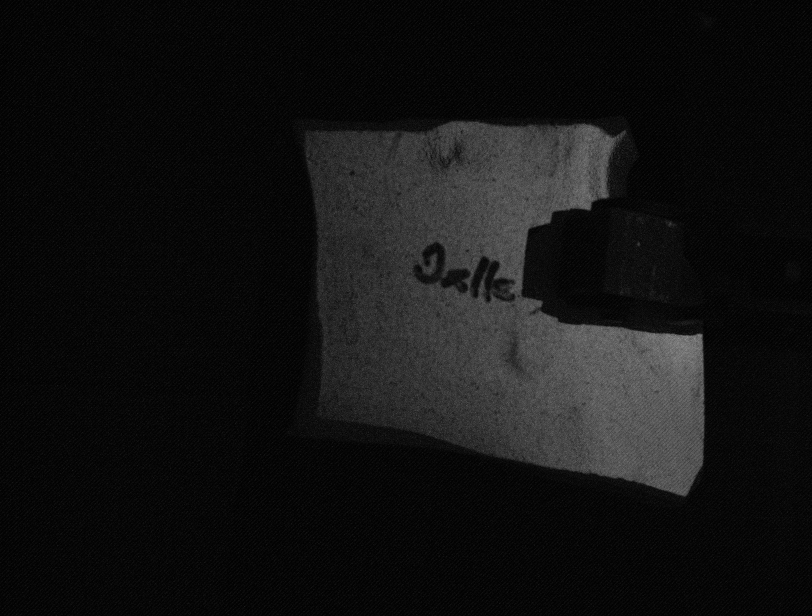
\includegraphics[width=.31\textwidth]{05_ergebnisse/ergSichtpruefungDurchLichtstreuung/spiegelbildAuswertungLichtstreuung/figures/keramikObjekt_2_combinePattern}};
		
		% Captions
		\node [below=0.2cm of img1] (cap1) {Brillenglas 1};
		\node [below=0.2cm of img2] (cap2) {Keramikobjekt 1};
		\node [below=0.2cm of img3] (cap3) {Keramikobjekt 2};		
	\end{tikzpicture}
\end{adjustbox}
\caption[Ergebnisbilder des Verfahrens \glqq Sichtprüfung durch Lichtstreuung\grqq ~bei der Spiegelbildauswertung]{Ergebnisbilder des Verfahrens \glqq Sichtprüfung durch Lichtstreuung\grqq ~bei der Spiegelbildauswertung}
		\label{tikz:abbCombinePatternPicturesSpLichtstreuung}
	\end{figure}
}

\noindent
Es wurde als Verknüpfungsmethode des Verfahrens die betragsmäßige Differenz gewählt, um die Bilder aus Abbildung \ref{tikz:abbCombinePatternPicturesSpLichtstreuung} zu erzeugen.
Auch hier ist die Begründung der höhere Kontrast zwischen den Prüfobjekten und dem Hintergrund.
In einem weiterem Schritt wurden die Bilder durch lokale Kontrastverbesserungen und geeigneter Kennlinientransformationen nachbearbeitet, um die Fehlstellen besser zu erkennen:

% Abbildung: Nachbearbeitung der Ergebnisbilder
{
	\begin{figure}[H]
		\centering
		\begin{adjustbox}{width=\textwidth}
	\begin{tikzpicture}[every node/.style={inner sep=0,outer sep=0}]
		% Bilder
		\node [anchor=north west] (img1) at (0,0) {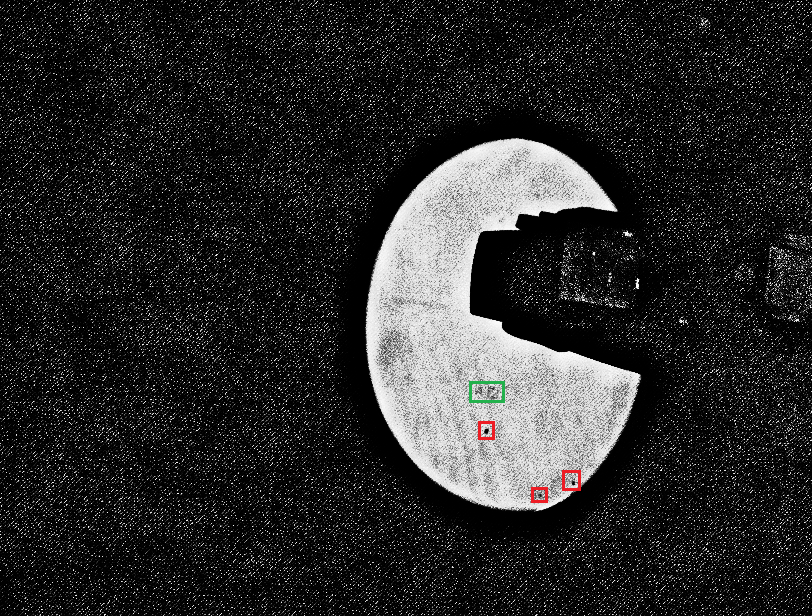
\includegraphics[width=.31\textwidth]{05_ergebnisse/ergSichtpruefungDurchLichtstreuung/spiegelbildAuswertungLichtstreuung/figures/brillenglas_1_verbessert}};
		\node [anchor=north west] (img2) at (0.345\textwidth,0) {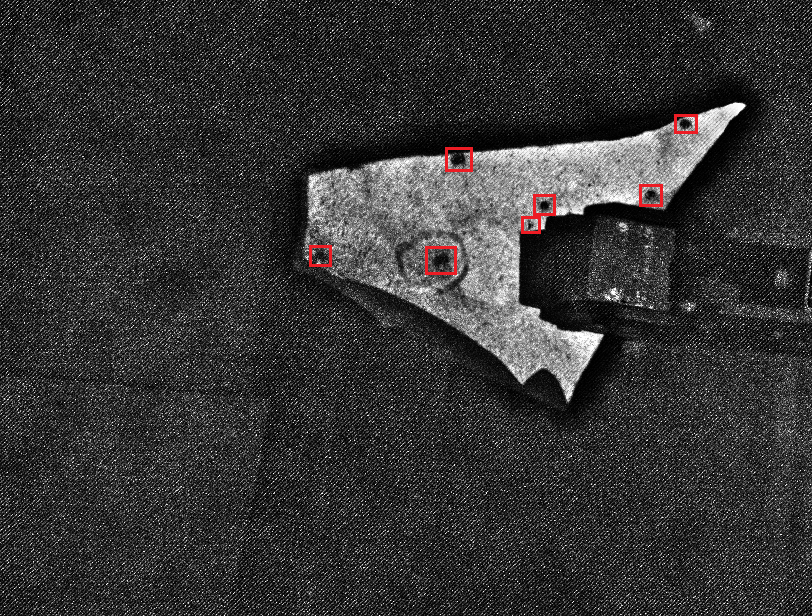
\includegraphics[width=.31\textwidth]{05_ergebnisse/ergSichtpruefungDurchLichtstreuung/spiegelbildAuswertungLichtstreuung/figures/keramikObjekt_1_verbessert}};
		\node [anchor=north west] (img3) at (0.69\textwidth,0) {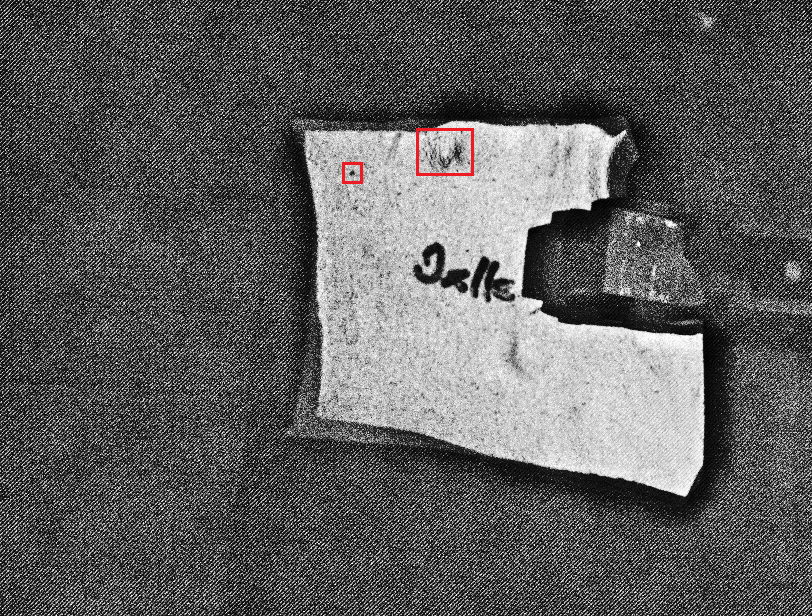
\includegraphics[width=.31\textwidth]{05_ergebnisse/ergSichtpruefungDurchLichtstreuung/spiegelbildAuswertungLichtstreuung/figures/keramikObjekt_2_verbessert}};
		
		% Captions
		\node [below=0.2cm of img1] (cap1) {Brillenglas 1};
		\node [below=0.2cm of img2] (cap2) {Keramikobjekt 1};
		\node [below=0.2cm of img3] (cap3) {Keramikobjekt 2};
	\end{tikzpicture}
\end{adjustbox}
\caption[Verbesserung der Ergebnisbilder]{Verbesserung der Ergebnisbilder. In Grün (bei Brillenglas 1): Gravur der Brillenglaskennzeichnung. In Rot: Kratzer, Pickel und ähnliche Be\-schä\-di\-gun\-gen der Oberfläche.}
		\label{tikz:abbNachbearbeitungSpLichtstreuung}
	\end{figure}
}

\noindent
In Abbildung \ref{tikz:abbNachbearbeitungSpLichtstreuung} sind die Fehlstellen in Rot markiert. 
Analog wie auch im vorherigen Abschnitt \ref{sub:durchlichtAuswertungLichtstreuung} erkennt man für Brillenglas 1 im grünen Rechteck eine Gravur des Markenzeichens auf der Oberfläche.
Für das Keramikobjekt 1 fallen einige dunkle Punkte im Objektbereich auf, welche durch sogenannte \glqq Pickel \grqq ~auf der Oberfläche entstehen.
Auf dem Keramikobjekt 2 befindet sich eine Delle, die im größeren roten Rechteck zu sehen ist.

%TODO Abschluss der Section?
}
}

%Deflektometrische Registrierung
{
	\FloatBarrier
    \section{Deflektometrische Registrierung}
    \label{sec:ergebnisseDeflektometrischeRegistrierung}
    Das Verfahren zur Bestimmung der deflektometrischen Registrierung wurde in Kapitel \ref{chp:deflektometrischeRegistrierung} eingeführt und bestimmt eine Zuordnung zwischen Bildschirm- und Kamerapunkten.
Nach Abschnitt \ref{sec:auswertungDeflektometrischeRegistrierung} lässt sich diese Zuordnung durch zwei Bilder darstellen und mittels Methoden aus der Bildverarbeitung auswerten.
Die Parameter zur Erzeugung der Muster nach Gleichung \ref{eq:monitormuster_mehrstufig} können in Tabelle \ref{tab:paramSichtpruefung} abgelesen werden.

\begin{table}[H]
	\centering
	\begin{tabular}{lll}
	\hline 
	\textbf{Beschreibung} & \textbf{Name} & \textbf{Wert} \\ 
	\hline 
	Amplitude (beeinflusst die Helligkeit) & $A_m$ & 127.5 \\
	Kontrast & $C_m$ & 1.0 \\
	Anzahl Perioden des ersten Muster & $N_p^1$ & 3 \\ 
	Anzahl Perioden des zweiten Muster & $N_p^2$ & 5 \\ 
	Anzahl Perioden des dritten Muster & $N_p^3$ & 7 \\  
	Anzahl Phasenverschiebungen jedes Musters & $N_{shift}$ & 4 \\ 
	Bildschirmbreite (in Pixel) & \acrshort{lwidth} & 1920 \\
	Bildschirmhöhe (in Pixel) & \acrshort{lheight} & 1080 \\
	\hline 
	\end{tabular} 
	\caption{Parameter der Streifenmuster für das Verfahren \glqq Bestimmung der deflektometrischen Registrierung\grqq.}
	\label{tab:paramDeflektometrischRegistrierung}
\end{table}

\noindent
Durch diese Parameter erhält man eine Sequenz aus 12 Mustern, die auf einem LCD-Bildschirm angezeigt und anschließend durch eine Kamera aufgenommen werden können.
Zur Kodierung der Oberfläche werden insgesamt 256 Helligkeitsstufen auf die Oberfläche abgebildet.

\p
Im Folgenden wird nur die deflektometrische Registrierung der Zeilen untersucht.
Die Ergebnisse der deflektometrischen Registrierung der Spalten liefert für die Auswertung ähnliche Ergebnisse, weshalb darauf verzichtet wird.

% Durchlichtauswertung
{
	\FloatBarrier
    \subsection{Durchlichtauswertung}
    \label{sub:durchlichtAuswertungDeflektometrischeRegistrierung}
    Wie auch im Abschnitt \ref{sec:ergebnisseSichtpruefungDurchLichtstreuung} soll das Verfahren zunächst mit der Durchlichtauswertung für transparente Objekte durchgeführt werden.
Für einen nachfolgenden Vergleich sollen mit dem Verfahren auch das Brillenglas 1 und das Brillenglas 2 aus Abbildung \ref{tikz:abbStreifenaufnahmen} ausgewertet werden.
Zusätzlich zu den beiden Objekten wird ein anderes Brillenglas mit diesem Verfahren untersucht.
Es wird der Aufbau aus dem linken Teilbild aus Abbildung \ref{tikz:abbAufbauFotos} verwendet und die Brillengläser auf der Halterung positioniert.
Die Brillengläser werden zur Demonstration bei der Anzeige eines einzelnen Streifenmusters nach den Parametern aus Tabelle \ref{tab:paramDeflektometrischRegistrierung} aufgenommen:

% Abbildung: Aufnahmen mit sinusoidalen Streifenmustern
{
	\begin{figure}[H]
		\centering
		\begin{adjustbox}{width=\textwidth}
	\begin{tikzpicture}[every node/.style={inner sep=0,outer sep=0}]
		% Bilder
		\node [anchor=north west] (img1) at (0,0) {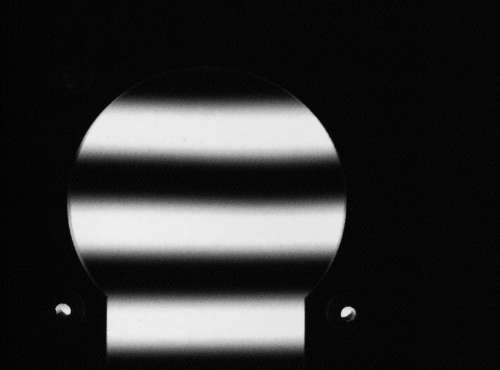
\includegraphics[width=.31\textwidth]{05_ergebnisse/ergDeflektometrischeRegistrierung/durchlichtAuswertungDeflektometrischeRegistrierung/figures/brillenglas_1_streifenmuster}};
		
		\node [anchor=north west] (img2) at (0.345\textwidth,0) {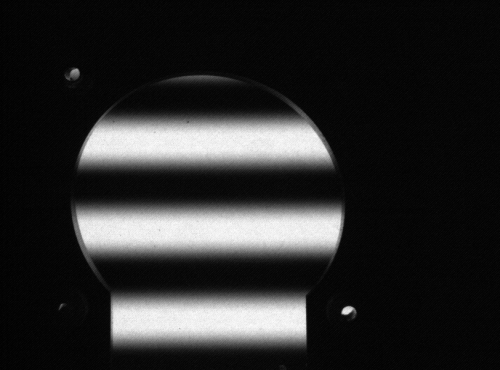
\includegraphics[width=.31\textwidth]{05_ergebnisse/ergDeflektometrischeRegistrierung/durchlichtAuswertungDeflektometrischeRegistrierung/figures/brillenglas_2_streifenmuster}};
		
		\node [anchor=north west] (img3) at (0.69\textwidth,0) {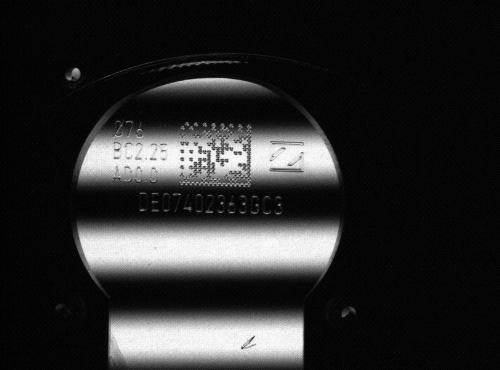
\includegraphics[width=.31\textwidth]{05_ergebnisse/ergDeflektometrischeRegistrierung/durchlichtAuswertungDeflektometrischeRegistrierung/figures/brillenglas_4_streifenmuster}};
		
		% Captions
		\node [below=0.2cm of img1] (cap1) {Brillenglas 1};
		\node [below=0.2cm of img2] (cap2) {Brillenglas 2};
		\node [below=0.2cm of img3] (cap3) {Brillenglas 4};			
	\end{tikzpicture}
\end{adjustbox}
\caption[Aufnahmen der Brillengläser bei der Durchlichtauswertung mit sinusoidalen Streifenmustern]{Aufnahmen der Brillengläser bei der Durchlichtauswertung mit sinusoidalen Streifenmustern}
		\label{tikz:abbSinusStreifenaufnahmen}
	\end{figure}
}

\noindent
Nach der Bestimmung der deflektometrischen Registrierung können daraus Bilder erstellt werden (siehe Definition \ref{def:graphDeflektometrischeRegistrierung}):

% Abbildung: Bilder der deflektometrische Registrierung der Zeilen
{
	\begin{figure}[H]
		\centering
		\begin{adjustbox}{width=\textwidth}
	\begin{tikzpicture}[every node/.style={inner sep=0,outer sep=0}]
		% Bilder
		\node [anchor=north west] (img1) at (0,0) {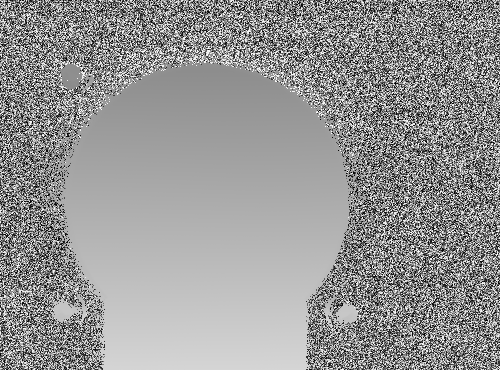
\includegraphics[width=.31\textwidth]{05_ergebnisse/ergDeflektometrischeRegistrierung/durchlichtAuswertungDeflektometrischeRegistrierung/figures/brillenglas_1_registrierung}};
		
		\node [anchor=north west] (img2) at (0.345\textwidth,0) {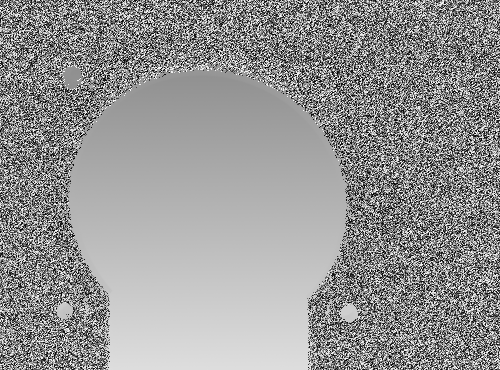
\includegraphics[width=.31\textwidth]{05_ergebnisse/ergDeflektometrischeRegistrierung/durchlichtAuswertungDeflektometrischeRegistrierung/figures/brillenglas_2_registrierung}};
		
		\node [anchor=north west] (img3) at (0.69\textwidth,0) {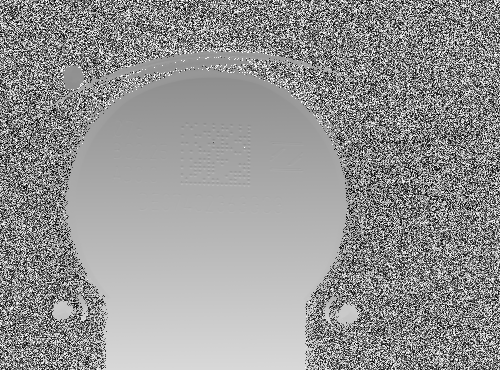
\includegraphics[width=.31\textwidth]{05_ergebnisse/ergDeflektometrischeRegistrierung/durchlichtAuswertungDeflektometrischeRegistrierung/figures/brillenglas_4_registrierung}};
		
		% Captions
		\node [below=0.2cm of img1] (cap1) {Brillenglas 1};
		\node [below=0.2cm of img2] (cap2) {Brillenglas 2};
		\node [below=0.2cm of img3] (cap3) {Brillenglas 4};			
	\end{tikzpicture}
\end{adjustbox}
\caption[Bilder der deflektometrischen Registrierung der Zeilen bei der Durchlichtauswertung]{Bilder der deflektometrischen Registrierung der Zeilen bei der Durchlichtauswertung.}
		\label{tikz:abbDeflectometricRegistrations}
	\end{figure}
}

\noindent
Zur Verdeutlichung der Ergebnisse des Verfahrens ist es sinnvoll die Ableitung der Bilder in Richtung der Zeilen zu bilden.
Mit Nachbearbeitung der Bilder der Ableitungen erhält man folgende Bilder:

% Abbildung: Bilder der deflektometrische Registrierung der Zeilen
{
	\begin{figure}[H]
		\centering
		\begin{adjustbox}{width=\textwidth}
	\begin{tikzpicture}[every node/.style={inner sep=0,outer sep=0}]
		% Bilder
		\node [anchor=north west] (img1) at (0,0) {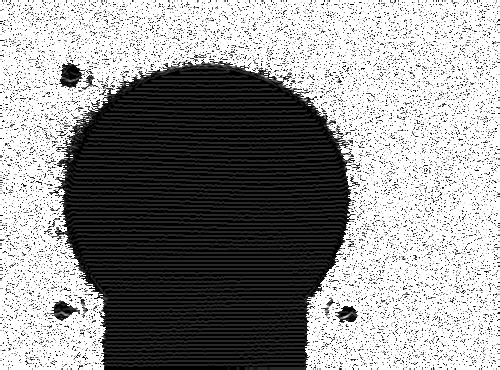
\includegraphics[width=.31\textwidth]{05_ergebnisse/ergDeflektometrischeRegistrierung/durchlichtAuswertungDeflektometrischeRegistrierung/figures/brillenglas_1_ableitung}};
		
		\node [anchor=north west] (img2) at (0.345\textwidth,0) {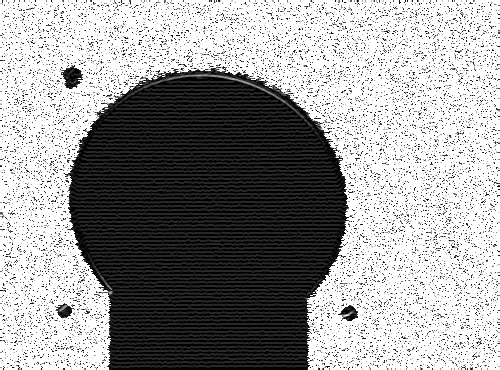
\includegraphics[width=.31\textwidth]{05_ergebnisse/ergDeflektometrischeRegistrierung/durchlichtAuswertungDeflektometrischeRegistrierung/figures/brillenglas_2_ableitung}};
		
		\node [anchor=north west] (img3) at (0.69\textwidth,0) {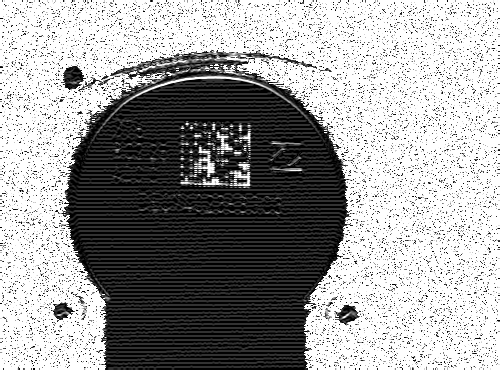
\includegraphics[width=.31\textwidth]{05_ergebnisse/ergDeflektometrischeRegistrierung/durchlichtAuswertungDeflektometrischeRegistrierung/figures/brillenglas_4_ableitung}};
		
		% Captions
		\node [below=0.2cm of img1] (cap1) {Brillenglas 1};
		\node [below=0.2cm of img2] (cap2) {Brillenglas 2};
		\node [below=0.2cm of img3] (cap3) {Brillenglas 4};			
	\end{tikzpicture}
\end{adjustbox}
\caption[Ableitung der deflektometrischen Registrierung der Zeilen bei der Durchlichtauswertung]{Ableitung der deflektometrischen Registrierung der Zeilen bei der Durchlichtauswertung.}
		\label{tikz:abbAbleitungRegistrierungDurchlicht}
	\end{figure}
}

%TODO Text
}

% Spiegelbildauswertung
{
	\FloatBarrier
    \subsection{Spiegelbildauswertung}
    \label{sub:spiegelbildAuswertungDeflektometrischeRegistrierung}
    Das Verfahren zur Bestimmung der deflektometrischen Registrierung konnte bestimmte Fehlstellen auch bei der Durchlichtauswertung sichtbar machen.
Allerdings sind schwächere Kratzer und Gravuren untergegangen.
Aus dem Grund wird zum Vergleich das Brillenglas 1 untersucht und durch den Aufbau für die Spiegelbildauswertung (siehe rechtes Teilbild aus Abbildung \ref{tikz:abbAufbauFotos}) geprüft, ob bessere Ergebnisse erzielt werden können.
Wie auch im Abschnitt \ref{sub:spiegelbildAuswertungLichtstreuung} kann für Brillenglas 1 der Rückseitenreflex durch den Polarisationsfilter und der Färbung nahezu vollständig vermieden werden.
Die Spiegelbildauswertung ermöglicht auch die Anwendung des Verfahrens für nicht-transparente spiegelnde Objekte, weshalb die Keramikobjekte 1 und 2 aus Abbildung \ref{tikz:abbStreifenaufnahmenSpLichtstreuung} zur Prüfung herangezogen werden.

\p
In Abbildung \ref{tikz:abbSinusStreifenmusterSpiegel} werden die Prüfobjekte unter der Spiegelung eines sinusoidalen Streifenmusters nach den Parametern aus Tabelle \ref{tab:paramDeflektometrischRegistrierung} dargestellt.

% Abbildung: Aufnahmen mit sinusoidalen Streifenmustern
{
	\begin{figure}[H]
		\centering
		\begin{adjustbox}{width=\textwidth}
	\begin{tikzpicture}[every node/.style={inner sep=0,outer sep=0}]
		% Bilder
		\node [anchor=north west] (img1) at (0,0) {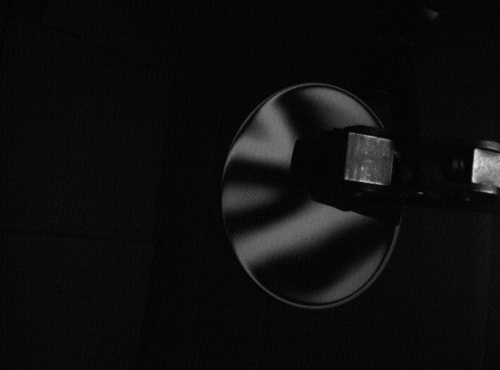
\includegraphics[width=.31\textwidth]{05_ergebnisse/ergDeflektometrischeRegistrierung/spiegelbildAuswertungDeflektometrischeRegistrierung/figures/brillenglas_1_streifenmuster}};
		
		\node [anchor=north west] (img2) at (0.345\textwidth,0) {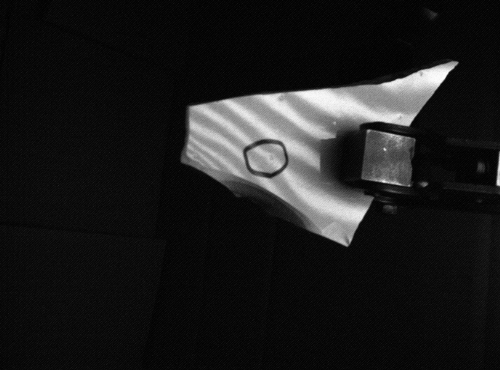
\includegraphics[width=.31\textwidth]{05_ergebnisse/ergDeflektometrischeRegistrierung/spiegelbildAuswertungDeflektometrischeRegistrierung/figures/keramikobjekt_1_streifenmuster}};
		
		\node [anchor=north west] (img3) at (0.69\textwidth,0) {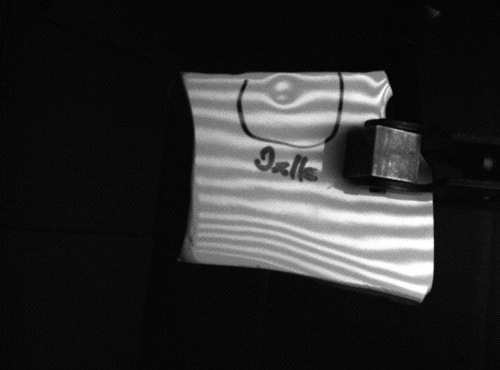
\includegraphics[width=.31\textwidth]{05_ergebnisse/ergDeflektometrischeRegistrierung/spiegelbildAuswertungDeflektometrischeRegistrierung/figures/keramikobjekt_2_streifenmuster}};
		
		% Captions
		\node [below=0.2cm of img1] (cap1) {Brillenglas 1};
		\node [below=0.2cm of img2] (cap2) {Keramikobjekt 1};
		\node [below=0.2cm of img3] (cap3) {Keramikobjekt 2};
	\end{tikzpicture}
\end{adjustbox}
\caption[Aufnahmen der Prüfobjekte unter Spiegelung der sinusoidalen Streifenmuster]{Aufnahmen der Prüfobjekte unter Spiegelung der sinusoidalen Streifenmuster}
		\label{tikz:abbSinusStreifenmusterSpiegel}
	\end{figure}
}

\noindent
Nach der Bestimmung der deflektometrischen Registrierungen der Prüfobjekte können daraus Bilder erstellt werden (siehe Definition \ref{def:graphDeflektometrischeRegistrierung}):

% Abbildung: Bilder der deflektometrische Registrierung der Zeilen
{
	\begin{figure}[H]
		\centering
		\begin{adjustbox}{width=\textwidth}
	\begin{tikzpicture}[every node/.style={inner sep=0,outer sep=0}]
		% Bilder
		\node [anchor=north west] (img1) at (0,0) {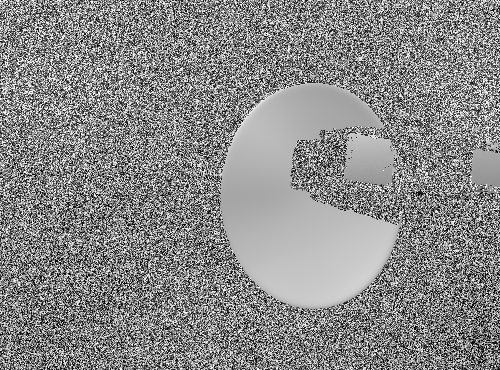
\includegraphics[width=.31\textwidth]{05_ergebnisse/ergDeflektometrischeRegistrierung/spiegelbildAuswertungDeflektometrischeRegistrierung/figures/brillenglas_1_registrierung}};
		
		\node [anchor=north west] (img2) at (0.345\textwidth,0) {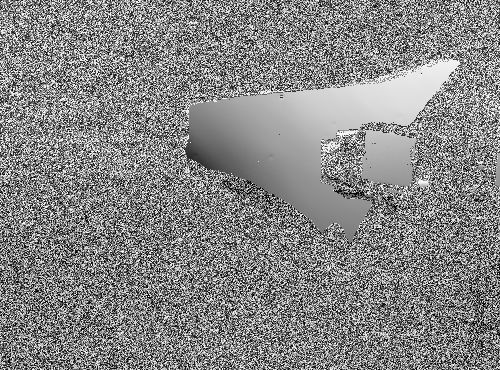
\includegraphics[width=.31\textwidth]{05_ergebnisse/ergDeflektometrischeRegistrierung/spiegelbildAuswertungDeflektometrischeRegistrierung/figures/keramikobjekt_1_registrierung}};
		
		\node [anchor=north west] (img3) at (0.69\textwidth,0) {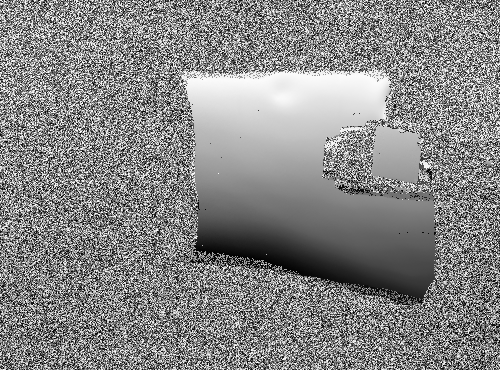
\includegraphics[width=.31\textwidth]{05_ergebnisse/ergDeflektometrischeRegistrierung/spiegelbildAuswertungDeflektometrischeRegistrierung/figures/keramikobjekt_2_registrierung}};
		
		% Captions
		\node [below=0.2cm of img1] (cap1) {Brillenglas 1};
		\node [below=0.2cm of img2] (cap2) {Keramikobjekt 1};
		\node [below=0.2cm of img3] (cap3) {Keramikobjekt 2};
	\end{tikzpicture}
\end{adjustbox}
\caption[Bilder der deflektometrischen Registrierung der Zeilen bei der Spiegelbildauswertung]{Bilder der deflektometrischen Registrierung der Zeilen bei der Spiegelbildauswertung.}
		\label{tikz:abbDeflectometricRegistrationsSpiegel}
	\end{figure}
}

\noindent
In den Bildern der deflektometrischen Zeilenregistrierung tauchen in den zu untersuchenden Objekten einzelne Bildpunkte auf, deren Grauwerte nicht zu der Umgebung passen.
Diese Ausreißer haben für die Oberflächenform keine größere Bedeutung und entstehen z. B. durch Messfehler, Fremdlicht oder die angestrahlte Abschirmung, die von innen Licht auf das Prüfobjekt reflektiert.
Durch Anwendung des Medianfilters zur Glättung des Bildes, kann man diese Störungen weitgehend entfernen.
Anschließend kann auch für diese Objekte zur Auswertung der deflektometrischen Registrierung die Ableitung der geglätteten Bilder in Richtung der Zeilen gebildet werden:

% Abbildung: Bilder der Ableitung der deflektometrische Registrierung der Zeilen
{
	\begin{figure}[H]
		\centering
		\begin{adjustbox}{width=\textwidth}
	\begin{tikzpicture}[every node/.style={inner sep=0,outer sep=0}]
		% Bilder
		\node [anchor=north west] (img1) at (0,0) {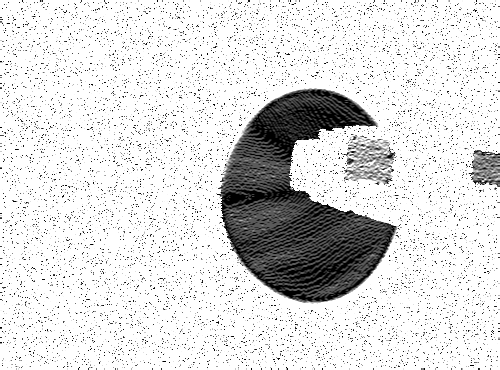
\includegraphics[width=.31\textwidth]{05_ergebnisse/ergDeflektometrischeRegistrierung/spiegelbildAuswertungDeflektometrischeRegistrierung/figures/brillenglas_1_ableitung}};
		
		\node [anchor=north west] (img2) at (0.345\textwidth,0) {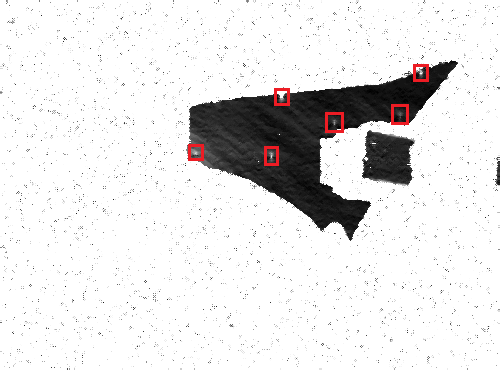
\includegraphics[width=.31\textwidth]{05_ergebnisse/ergDeflektometrischeRegistrierung/spiegelbildAuswertungDeflektometrischeRegistrierung/figures/keramikobjekt_1_ableitung}};
		
		\node [anchor=north west] (img3) at (0.69\textwidth,0) {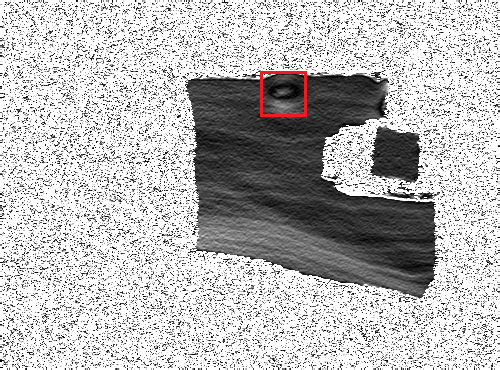
\includegraphics[width=.31\textwidth]{05_ergebnisse/ergDeflektometrischeRegistrierung/spiegelbildAuswertungDeflektometrischeRegistrierung/figures/keramikobjekt_2_ableitung}};
		
		% Captions
		\node [below=0.2cm of img1] (cap1) {Brillenglas 1};
		\node [below=0.2cm of img2] (cap2) {Keramikobjekt 1};
		\node [below=0.2cm of img3] (cap3) {Keramikobjekt 2};
	\end{tikzpicture}
\end{adjustbox}
\caption[Ableitungen der Bilder der deflektometrischen Registrierung der Zeilen bei der Spiegelbildauswertung]{Ableitung der Bilder der deflektometrischen Registrierung der Zeilen bei der Spiegelbildauswertung.}
		\label{tikz:abbAbleitungRegistrierungSpiegel}
	\end{figure}
}

\noindent
Genau wie bei der Durchlichtauswertung durch dieses Verfahren, lassen sich bei dem Brillenglas 1 in Abbildung \ref{tikz:abbAbleitungRegistrierungSpiegel} keine größeren Auffälligkeiten feststellen.
Es lassen sich demnach nicht wie im Abschnitt \ref{sub:spiegelbildAuswertungLichtstreuung} Fehlstellen oder die Gravur der Brillenkennzeichnung erkennen.
Auf den Keramikobjekten 1 und 2 erkennt man Abweichungen von den Krümmungsverläufen der Oberfläche.
In Abbildung \ref{tikz:abbAbleitungRegistrierungSpiegel} sind diese Auffälligkeiten durch rote Rechtecke markiert.
Beim Keramikobjekt 1 handelt es sich hierbei um sogenannte  \glqq Pickel\grqq ~auf der Oberfläche.
Auf der Oberfläche des Keramikobjekts 2 befindet sich im roten Rechteck eine Delle bzw. Wölbung.

\p
Als Alternative zur Auswertung der deflektometrischen Registrierung über die Ableitung, wird eine Auswertung über die Krümmungsberechnung durch den sogenannten \glqq Mexican Hat\grqq -Operator\footnote{
Der \glqq Mexican Hat\grqq -Operator bzw. der Laplace of Gaussian kann verwendet werden um die zweite Ableitung eines Bildes zu berechnen.
} durchgeführt:

% Abbildung: Bilder des Mexican Hat Filter angewandt auf die deflektometrische Registrierung der Zeilen
{
	\begin{figure}[H]
		\centering
		\begin{adjustbox}{width=\textwidth}
	\begin{tikzpicture}[every node/.style={inner sep=0,outer sep=0}]
		% Bilder
		\node [anchor=north west] (img1) at (0,0) {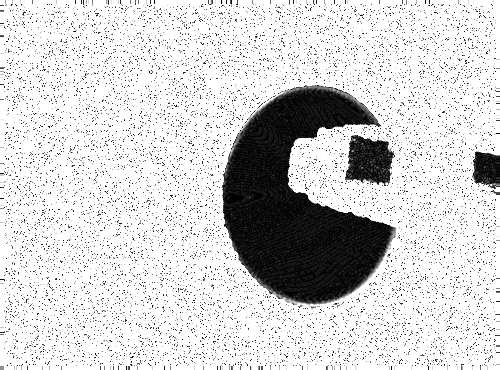
\includegraphics[width=.31\textwidth]{05_ergebnisse/ergDeflektometrischeRegistrierung/spiegelbildAuswertungDeflektometrischeRegistrierung/figures/brillenglas_1_mexican}};
		
		\node [anchor=north west] (img2) at (0.345\textwidth,0) {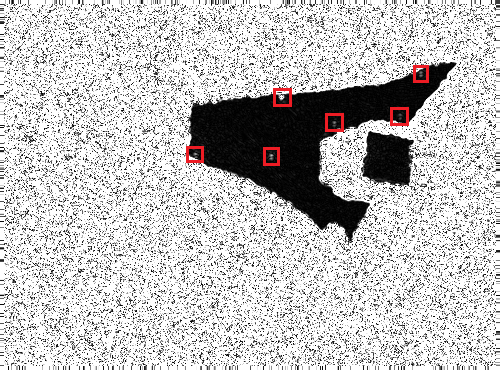
\includegraphics[width=.31\textwidth]{05_ergebnisse/ergDeflektometrischeRegistrierung/spiegelbildAuswertungDeflektometrischeRegistrierung/figures/keramikobjekt_1_mexican}};
		
		\node [anchor=north west] (img3) at (0.69\textwidth,0) {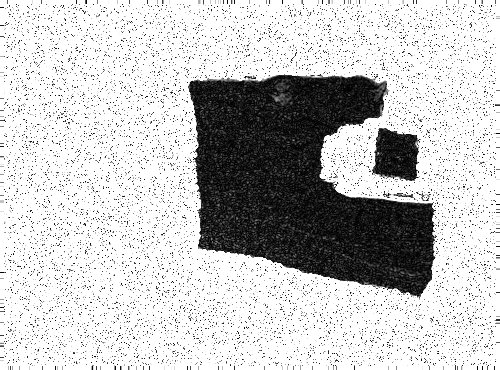
\includegraphics[width=.31\textwidth]{05_ergebnisse/ergDeflektometrischeRegistrierung/spiegelbildAuswertungDeflektometrischeRegistrierung/figures/keramikobjekt_2_mexican}};
		
		% Captions
		\node [below=0.2cm of img1] (cap1) {Brillenglas 1};
		\node [below=0.2cm of img2] (cap2) {Keramikobjekt 1};
		\node [below=0.2cm of img3] (cap3) {Keramikobjekt 2};
	\end{tikzpicture}
\end{adjustbox}
\caption[Mexican Hat-Filter angewandt auf die Bilder der deflektometrischen Registrierung der Zeilen]{Mexican Hat-Filter angewandt auf die Bilder der deflektometrischen Registrierung der Zeilen.}
		\label{tikz:abbMexicanHatRegistrierung}
	\end{figure}
}

\noindent
Auch in Abbildung \ref{tikz:abbMexicanHatRegistrierung} erkennt man im Brillenglas keine Abweichungen der Oberflächen\-krümmung.
Auf den Keramikobjekten 1 und 2 erkennt man an den in Abbildung \ref{tikz:abbAbleitungRegistrierungSpiegel} markierten Fehlstellen auch Auffälligkeiten in Abbildung \ref{tikz:abbMexicanHatRegistrierung}.
}
}

%Diskussion
{
	\FloatBarrier
    \section{Diskussion}
    \label{sec:diskussion}
    Im Folgenden sollen die beschriebenen Ergebnisse aus den vorherigen Abschnitten \ref{sec:ergebnisseSichtpruefungDurchLichtstreuung} und \ref{sec:ergebnisseDeflektometrischeRegistrierung} aufgegriffen und bewertet werden.
Das Ziel ist es abhängig vom Anwendungsfall ein passendes Verfahren vorzuschlagen und die Schwächen und Stärken der Verfahren darzulegen.

\p
Für das Verfahren \glqq Sichtprüfung durch Lichtstreuung\grqq ~fällt im Abschnitt \ref{sec:ergebnisseSichtpruefungDurchLichtstreuung} auf, dass es sich besonders gut für die Durchlichtauswertung von transparenten Prüfobjekten eignet.
Es ist möglich bereits sehr kleine Defekte, wie z. B. sehr leichte Kratzer oder Laser-Gravuren auf den Objektoberflächen zu erkennen (siehe Abbildung \ref{tikz:abbErkennbareKleineDefekteLichtstreuung}).

% Abbildung: Erkennbare kleine Defekte
{
	\begin{figure}[H]
		\centering
		\begin{tikzpicture}[every node/.style={inner sep=0,outer sep=0}]

	\node [anchor=north east] (img1) at (-0.03\textwidth,0) {\includegraphics[width=.4\textwidth]{05_ergebnisse/ergDiskussion/figures/lasergravur}};
	\node [below=0.2cm of img1] {Ausschnitt von Brillenglas 1};
	\node [anchor=north west] (img2) at (0.03\textwidth,0) {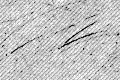
\includegraphics[width=.4\textwidth]{05_ergebnisse/ergDiskussion/figures/polierfehler}};
	\node [below=0.2cm of img2] {Ausschnitt von Brillenglas 2};
	
\end{tikzpicture}
\caption[Erkennbare kleine Defekte oder Laser-Gravur]{Erkennbare kleine Defekte oder Laser-Gravuren durch Durchlichtauswertung mit Verfahren \glqq Sichtprüfung durch Lichtstreuung\grqq ~(siehe Kapitel \ref{chp:sichtpruefungDurchLichtstreuung}) Linkes Teilbild: Erkennbare Lasergravur, Rechtes Teilbild: Leichte Kratzer durch Fehler bei der Polierung}
		\label{tikz:abbErkennbareKleineDefekteLichtstreuung}
	\end{figure}
}

\noindent
Außerdem ist es möglich für transparente Objekte durch die Durchlichtauswertung auch Defekte im Objekt, wie z. B. Lufteinschlüsse in Gläsern festzustellen.
Dies konnte allerdings nicht nachgeprüft werden, da solche Defekte in den zur Verfügung stehenden Prüfobjekten nicht vorhanden waren.

\p
Für nicht-transparente Prüfobjekte kann das Verfahren \glqq Sichtprüfung durch Lichtstreuung\grqq ~durch eine Spiegelbildaufwertung ebenfalls verwertbare Bilder erzeugen um Defekte zu detektieren, allerdings gibt es hierbei schon erste Probleme.
Eine große Schwäche des Verfahrens ist die Abhängigkeit von Oberflächenbeschriftungen oder -aufdrucken.
Da stets Grauwerte der Kamerabilder verknüpft werden beeinflussen unterschiedliche Farben auf der Oberfläche das Ergebnis (siehe Abbildung \ref{img:delleBeschriftung}).
Das gleiche Phänomen lässt sich auch beobachten wenn das Objekt abhängig von der Position unterschiedlich stark reflektierend ist.

% Abbildung: Beschriftung Delle
{
	\begin{figure}[H]
		\centering
		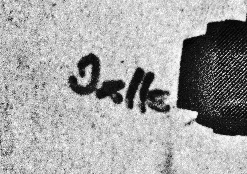
\includegraphics[width=0.4\textwidth]{05_ergebnisse/ergDiskussion/figures/delleBeschriftung}
		\caption[Sichtbare Beschriftung nach Anwendung des Verfahrens aus Kapitel \ref{chp:sichtpruefungDurchLichtstreuung}]{Sichtbare Beschriftung \glqq Delle\grqq ~nach Anwendung des Verfahren \glqq Sichtprüfung durch Lichtstreuung\grqq auf Keramikobjekt 2. Ausschnitt aus Abbildung \ref{tikz:abbNachbearbeitungSpLichtstreuung}}
		\label{img:delleBeschriftung}
	\end{figure}
}

\noindent
Dieser Einfluss kann zu Problemen in der nachfolgenden Auswertung des Ergebnisbilds durch herkömmliche Bildverarbeitungsalgorithmen führen.
Für dieses Verfahren ist es also notwendig, dass das Prüfobjekt einfarbig und ohne Beschriftungen vorliegt.
Außerdem sollte das Prüfobjekt an allen zu untersuchenden Stellen das Licht gleich stark reflektieren.
Damit können kleinere Defekte, wie z. B. Oberflächenpickel oder Kratzer in Brillengläsern detektiert werden.
Größere Defekte wie z. B. die Delle auf der Oberfläche des Keramikobjekts 2 (siehe Abbildung \ref{tikz:abbNachbearbeitungSpLichtstreuung}) sind hingegen schwerer zu identifizieren.
Dieselben Effekte in den Ergebnisbildern wie bei Dellen können auch bei stärker gekrümmten Objekten oder an matten Stellen auftreten.

\p
Die deflektometrische Registrierung erzeugt lediglich Zuordnungsinformationen die durch spezielle Algorithmen weiterverarbeitet werden muss um Untersuchungen der Oberfläche zu treffen.
In dem Abschnitt \ref{sec:ergebnisseDeflektometrischeRegistrierung} wurde zunächst ein Bild aus der  deflektometrischen Registrierung der Zeilen erzeugt, dass man Bildverarbeitungsalgorithmen anwenden kann um bestimmte Auffälligkeiten hervorheben zu können.
Allerdings verliert man nach dem vorgestellten Ansatz eventuell Informationen über sehr kleine Defekte, da bei der Bilderzeugung je nach verwendeter Farbtiefe mehrere Zeilenpositionen demselben Grauwert zugeordnet werden.
Man verliert kleine Details der deflektometrischen Registrierung, das macht es schwieriger sehr kleine Abweichungen der Reflexionen, wie z. B. Kratzer oder Laser-Gravuren zu erkennen.
Die tatsächlichen Reflexionsabweichungen sind bei der Durchlichtauswertung kleiner als bei dem Spiegelbild.
Es lässt sich auch in Abbildung \ref{tikz:abbAbleitungRegistrierungDurchlicht} erkennen, dass sich das Verfahren für die Durchlichtauswertung von Brillengläsern nur begrenzt eignet.
Auch die Auswertung des Spiegelbilds von Brillenglas 1 zeigt keine Auffälligkeiten, da die Kratzer und Laser-Gravuren die Reflexion des Lichts nur minimal beeinflussen (siehe Abbildung \ref{tikz:abbAbleitungRegistrierungSpiegel}).

\p
Für die Spiegelbildauswertung durch Bestimmung der deflektometrischen Registrierung der Zeilen sind für die untersuchten Keramikobjekte bessere Ergebnisse zu erkennen (siehe Abbildung \ref{tikz:abbErkennbareDefekteRegistrierung}).

% Abbildung: Erkennbare Defekte
{
	\begin{figure}[H]
		\centering
		\begin{tikzpicture}[every node/.style={inner sep=0,outer sep=0}]

	\node [anchor=north east] (img1) at (-0.03\textwidth,0) {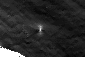
\includegraphics[width=.4\textwidth]{05_ergebnisse/ergDiskussion/figures/pickel}};
	\node [below=0.2cm of img1, align=center] {Ausschnitt von Keramikobjekt 1 \\ aus Abbildung \ref{tikz:abbAbleitungRegistrierungSpiegel}};
	\node [anchor=north west] (img2) at (0.03\textwidth,0) {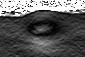
\includegraphics[width=.4\textwidth]{05_ergebnisse/ergDiskussion/figures/delle}};
	\node [below=0.2cm of img2, align=center] {Ausschnitt von Keramikobjekt 2 \\ aus Abbildung \ref{tikz:abbAbleitungRegistrierungSpiegel}};
	
\end{tikzpicture}
\caption[Erkennbare Oberflächendefekte durch deflektometrische Registrierung]{Erkennbare Oberflächendefekte durch Ableitung der deflektometrischen Registrierung. Linkes Teilbild: Oberflächenpickel, Rechtes Teilbild: Delle in der Oberfläche}
		\label{tikz:abbErkennbareDefekteRegistrierung}
	\end{figure}
}

\noindent
Ein großer Vorteil der Auswertung über die deflektometrische Registrierung ist die Unabhängigkeit von Oberflächenbeschriftungen oder -aufdrucken.
Es ist also möglich Objekte mit verschiedenen Farben oder Lackierungen zu prüfen.
Außerdem erhält man durch das Verfahren tatsächliche Krümmungsinformationen der Objektoberfläche die ausgewertet werden können.
Eine Schwäche der deflektometrischen Registrierung ist die Empfindlichkeit gegenüber Fremdlichteinwirkungen oder störende Reflexionen, wie z. B. den Rückseitenreflex bei spiegelnden Objektoberflächen (siehe Abbildung \ref{tikz:abbRückseitenreflexRegistrierung}).

% Abbildung: Rückseitenreflex Registrierung
{
	\begin{figure}[H]
		\centering
		\input{05_ergebnisse/ergDiskussion/figures/abbRückseitenreflexRegistrierung}
		\label{tikz:abbRückseitenreflexRegistrierung}
	\end{figure}
}

\noindent
Durch die Überlagerung der Reflexionen im Kamerabild ist es nicht länger möglich die Dekodierung korrekt durchzuführen.
Es kommt an manchen Stellen zu Fehlern und Phasensprüngen.
Dadurch wird auch die Auswertung des Bildes keine nützlichen Ergebnisse mehr erbringen können.

\p
Die Problematik des Rückseitenreflexes trifft auch auf das Verfahren \glqq Sichtprüfung durch Lichtstreuung\grqq ~zu.
Durch die überlagerten Streifenmuster kann es passieren, dass fehlerhafte Strukturen durch das Verfahren entstehen (siehe Abbildung \ref{tikz:abbRückseitenreflexLichtstreuung}).

% Abbildung: Rückseitenreflex Lichtstreuung
{
	\begin{figure}[H]
		\centering
		\input{05_ergebnisse/ergDiskussion/figures/abbRückseitenreflexLichtstreuung}
		\label{tikz:abbRückseitenreflexLichtstreuung}
	\end{figure}
}

\noindent
Durch die bisherigen Ausführungen lassen sich in den vorgestellten Verfahren Stärken und Schwächen erkennen.
Ausgehend davon soll nun die Eignung der Verfahren für spezielle Anwendungen vermittelt werden.
Aus Abbildungen \ref{tikz:abbRückseitenreflexRegistrierung} und \ref{tikz:abbRückseitenreflexLichtstreuung} lässt sich schließen, dass transparente Objekte durch den Rückseitenreflex nicht für die Spiegelbildauswertung mit den vorgestellten Verfahren geeignet sind.
Aufgrund der hohen Präzision bei der Durchlichtauswertung bietet sich deshalb besonders das Verfahren \glqq Sichtprüfung durch Lichtstreuung\grqq an, wenn die qualitative Sichtprüfung des Objekts ausreichend ist.
Sobald weitere Informationen, wie z. B. die Oberflächenkrümmung erforderlich sind, sollte für die Objekte die deflektometrische Registrierung des Spiegelbilds bestimmt werden.
Dabei muss dann auch das Problem des Rückseitenreflexes behandelt werden.

\p
Es wird ersichtlich, dass das Verfahren zur Auswertung der deflektometrischen Registrierung bessere Ergebnisse für nicht-transparente spiegelnde Objekte bei der Spiegelbildanalyse erzielen kann.
Im Vergleich zum Verfahren \glqq Sichtprüfung durch Lichtstreuung\grqq ist die deflektometrische Registrierung besser geeignet für stärker gekrümmte oder lackierte Objekte.
Die deflektometrische Registrierung kann durch weitere Verarbeitungen auch genutzt werden um die Oberfläche des Prüfobjekts zu rekonstruieren.
Diese Möglichkeiten machen die deflektometrische Registrierung zu einer nützlichen Information über Oberflächen zur Erfassung von Oberflächendefekten für spiegelnde Objekte.
}